%%!TEX root=../main.tex

\section{Evaluation}
Now, we investigate the performance of our various method. As mentioned before, the RNN method mainly used to predict the location of tennis balls whereas MLP method and SVM mainly used to classify the tennis whether be out of the bound or not. So we use different evaluation metric on different methods.
\subsection{Prediction of location}
For RNN method, because it predict the location of the tennis balls so we select two evaluation indicators: mean square error (MSE) and mean absolute error (MAE). The formula of mean square error is as follows:
\begin{equation}
    \frac{1}{m} \sum_{i=1}^{m} (y_{test}^{(i)}-\hat{y}_{test}^{(i)})^2   
\end{equation}
we can get the result as shown in the figure \ref{MSE}below. From the figure, we can see that the value of MSE changes with the increase in the number of epochs. Within 100 epochs, the value of MSE drops sharply, and up to 250 epochs, there is basically no fluctuation, which means that the model has been fitted.

\begin{figure}[ht]
\centering
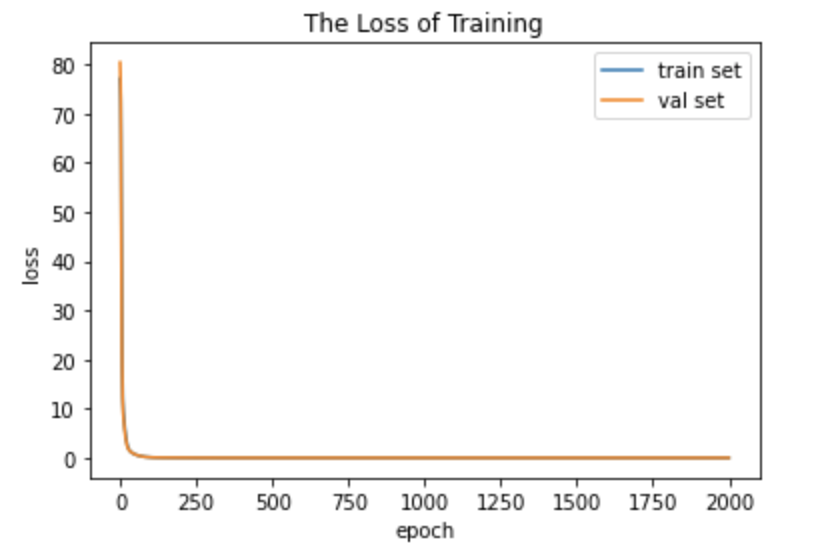
\includegraphics[width=3in]{\FIGDIR/P10_MSE.png}
\caption{The MSE of training}
\label{MSE}
\end{figure}
Another evaluation standard is MAE. Its principle is: to minimize the distance between the true value and the predicted result, we can directly subtract the absolute value, add m times and divide by M to find the average distance. The expression is as follows:
\begin{equation}
 \frac{1}{m} \sum_{i=1}^{m} |y_{test}^{(i)}-\hat{y}_{test}^{(i)}|   
\end{equation}
Figure \ref{mae} shows the result. The figure shows that the value of MAE decreases with the increase in the number of epochs. The curve changes are basically similar to the MSE curve, which proves the previous conclusion that the model has been fitted.

\begin{figure}[ht]
\centering
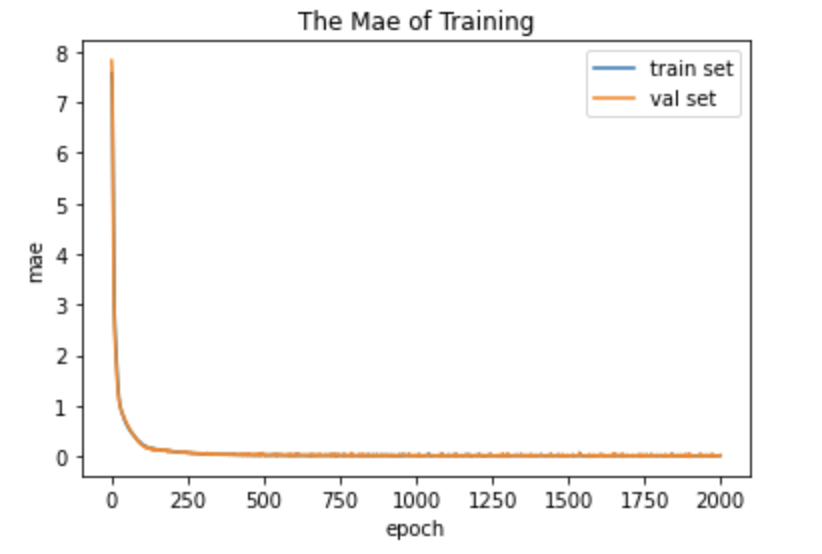
\includegraphics[width=3in]{\FIGDIR/P11_MAE.png}
\caption{The MAE of training}
\label{MAE}
\end{figure}
We use the trained model and the input value of the test set to predict. Figure \ref{rnn result}  shows the predicted results of the test set and the actual label value. From the figure, we can see that each predicted value and the actual value coincide, and the centroid of the predicted value basically coincides with the actual value. When we use MSE and Mae to evaluate the performance of model on test set, the MSE value is 2.1721e-04, MAE value is 0.0119.

\begin{figure}[ht]
\centering
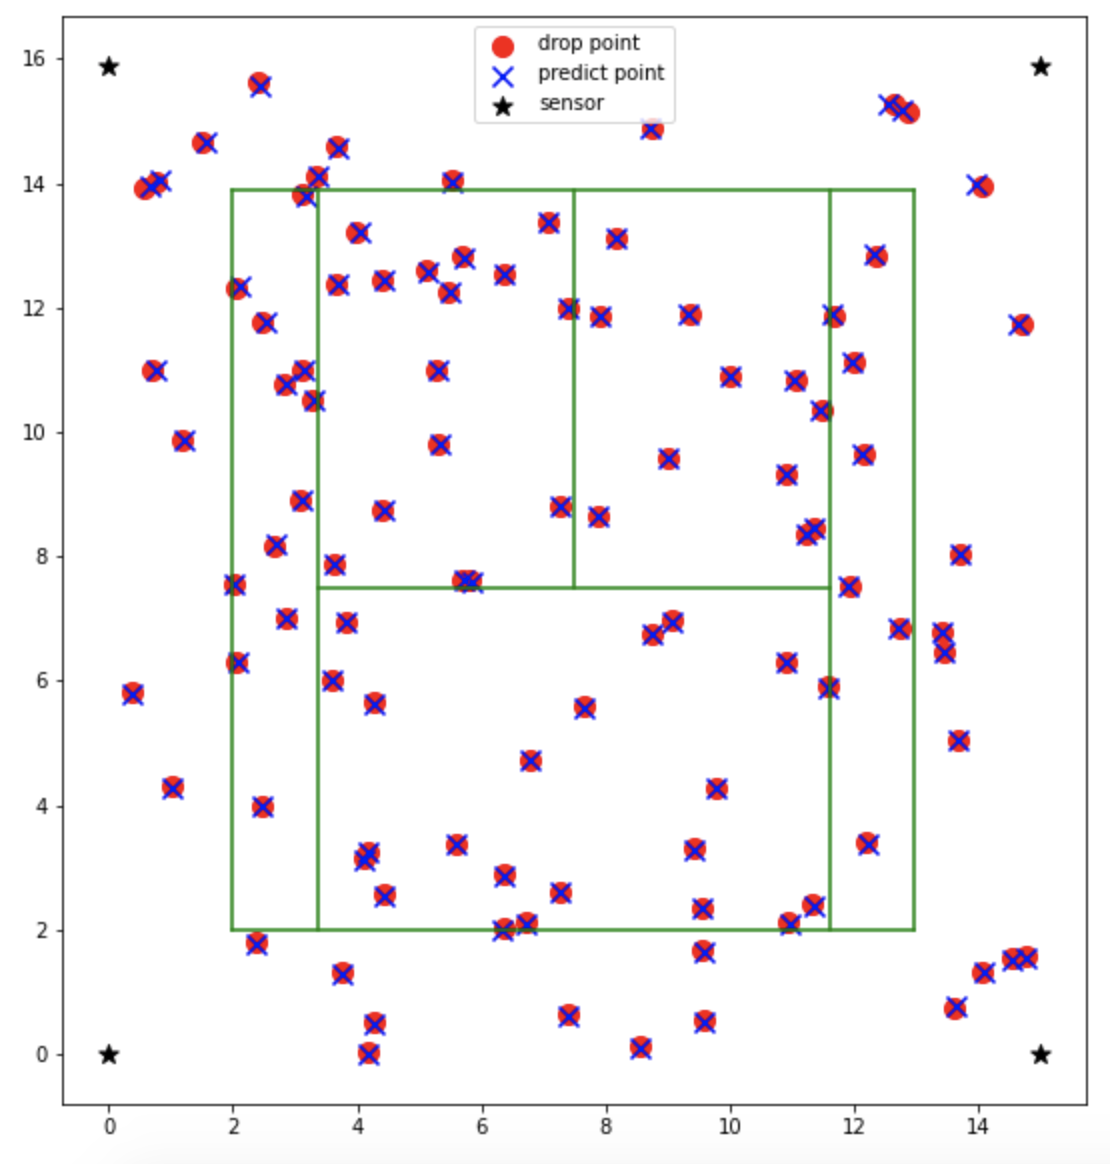
\includegraphics[width=3.5in]{\FIGDIR/P12_Prediction.png}
\caption{The Comparison of Prediction Values and Labels}
\label{rnn result}
\end{figure}

\subsection{Classification of legal or not}
We use MLP method and SVM to classify the tennis balls whether it is out of bound or not.

We print out the history of the loss value for the training model and make a plot, we can get the result as shown in the following figure. As shown in the figure \ref{loss}, with the increase in the number of epochs, the loss gradually decreases. After 800 epoch, the loss of the validation set is only 0.0454. 

\begin{figure}[ht]
\centering
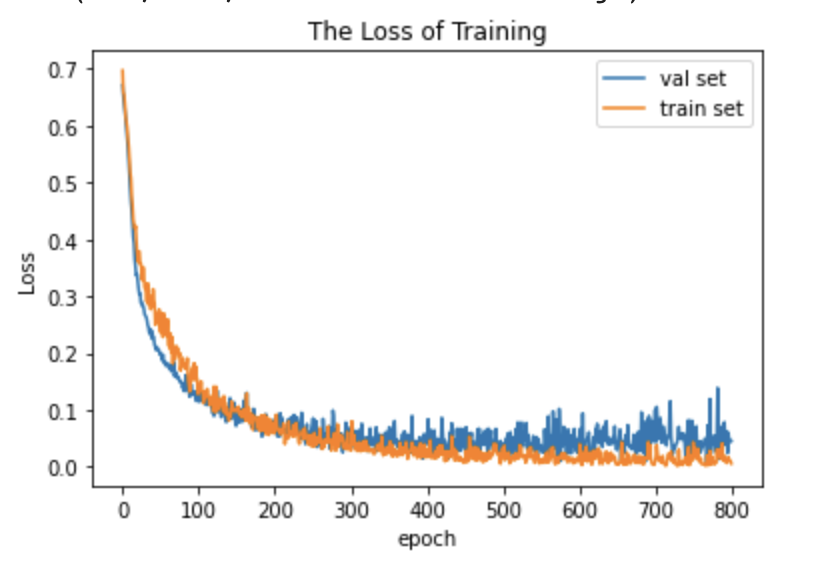
\includegraphics[width=3in]{\FIGDIR/P14_Loss.png}
\caption{The Loss of Training}
\label{loss}
\end{figure}
Use the same method to print the accuracy graph, as shown in the figure \ref{acc}. As the number of epoch increases, the accuracy gradually increases. Finally, through 800 epoch the accuracy of the validation set can reach 98.75\%.

\begin{figure}[ht]
\centering
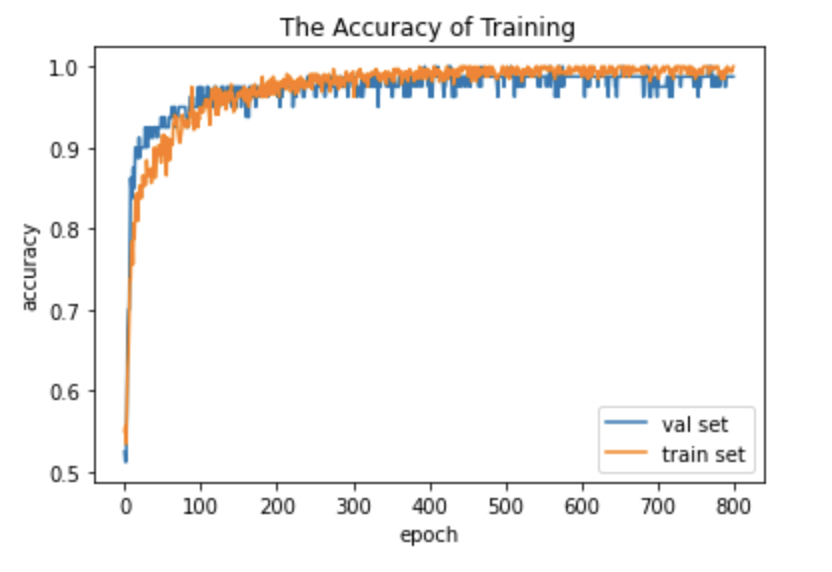
\includegraphics[width=3in]{\FIGDIR/P15_Acc.png}
\caption{The Accuracy of Training}
\label{acc}
\end{figure}

For SVM,we use the parameter which mentioned in the last section and then use test set to predict the label,the final accuracy is 96\%.

We further applied the values of the test set to the trained model. By using the evaluate function, the loss of the model on the test set is 0.2388, and the accuracy could reach 97\%.

To better evaluate our MLP model, we introduced the confusion matrix, F1-Score, and the ROC curve. The predicted result and the actual value can be composed of four situations:

True Positive (TP): the actual value is 0 and the predicted value is 0;

False Negative (FN): The actual value is 0, the predicted value is 1;

False Positive (FP): the actual value is 1 and the predicted value is 0;

True Negative (TN): The actual value is 1 and the predicted value is 1.
The confusion matrix is a situation analysis table that summarizes the prediction results of the classification model. In the form of a matrix, by using the TP, FN, FP and TN to record and summarize the dataset according to the two criteria of real classification and classification judgment made by the classification model. The result is shown figure \ref{confusion matrix} and \ref{confusion matrix of SVM}:

\begin{figure}[ht]
\centering
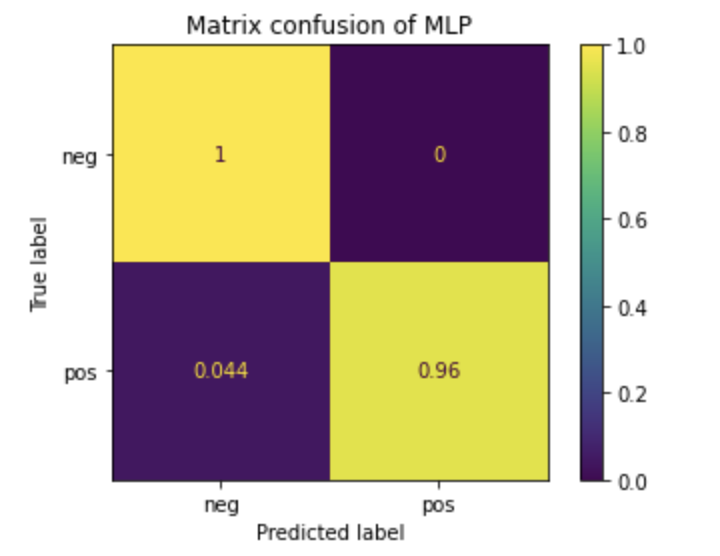
\includegraphics[width=2in]{\FIGDIR/P17_Confusion.png}
\caption{The Confusion Matrix of MLP}
\label{confusion matrix}
\end{figure}\begin{figure}[ht]
\centering
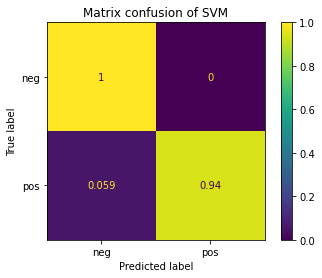
\includegraphics[width=2in]{\FIGDIR/confusionsvm.png}
\caption{The Confusion Matrix of SVM}
\label{confusion matrix of SVM}
\end{figure}
As described above, by using the definition of TP, FN, FP and TN, the $Precison$ could be expressed as:
\begin{equation}
    Precison=\frac{TP}{TP+FP}
\end{equation}
the $Recall$ could be written as:
\begin{equation}
    Recall=\frac{TP}{TP+FN}
\end{equation}
From the above formulas, we could have:
\begin{equation}
    F1-Score = \frac{2\cdot Precison \cdot Recall }{Precison + Recall}
\end{equation}
For a certain classification, F1 score combines precision and recall as the judgment criteria. From the formula, it can be seen that the larger the F1 score value is, the stronger the classification ability of the model is. As shown in the following figure \ref{f1} and \ref{f1s}, the F1-Score of the MLP model and SVM was calculated. For class 0, the F1-Score is 0.96 and class 1 is 0.98. Both values are close to 1 which means the built MLP model has a strong ability of classification.

\begin{figure}[ht]
\centering
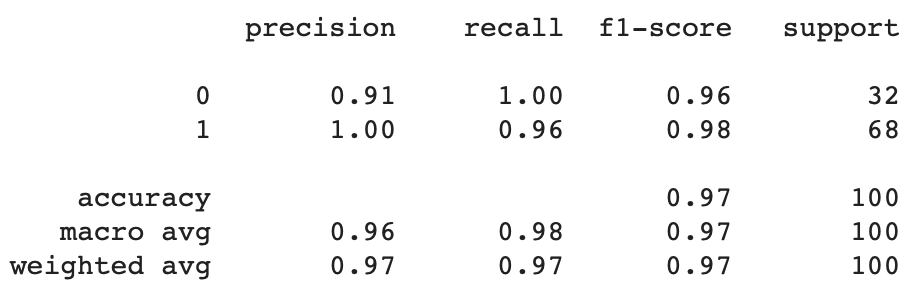
\includegraphics[width=3in]{\FIGDIR/P16_F1.png}
\caption{The F-1 Score of MLP}
\label{f1}
\end{figure}
\begin{figure}[ht]
\centering
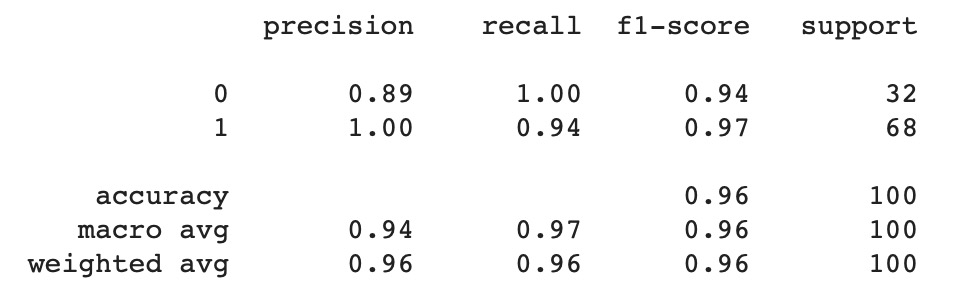
\includegraphics[width=3in]{\FIGDIR/f1svm.jpg}
\caption{The F-1 Score of SVM}
\label{f1s}
\end{figure}
The ROC curve represents the corresponding changes in the proportion of True Positive Rate (TPR) and False Positive Rate (FPR) of the model for the correct classification of real Positive samples and the proportion of False Positive Rate (FPR) for the negative samples when the selected classification threshold is gradually increased, with the horizontal axis representing FPR and the vertical axis representing TPR. Generally speaking, the closer the ROC curve of the model is to the upper left, the better the performance of the model. As shown in figure \ref{roc} and \ref{rocs}, the curve of both the MLP model and SVM is close to the upper left of entire plot.

\begin{figure}[ht]
\centering
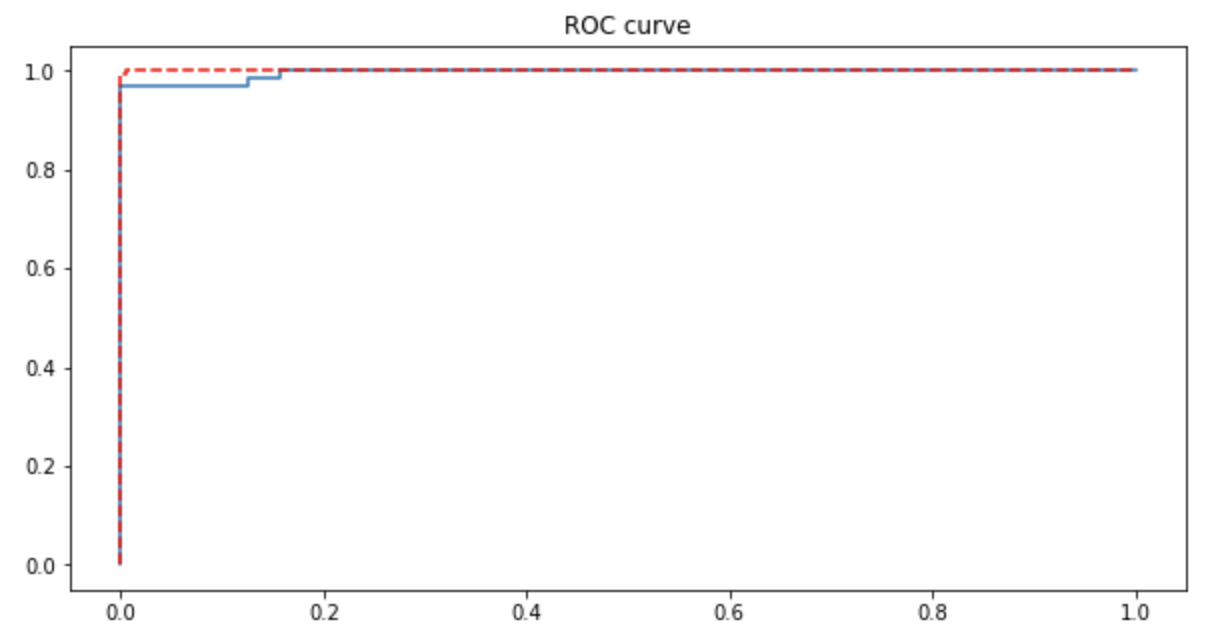
\includegraphics[width=3in]{\FIGDIR/P18_ROC.png}
\caption{The Roc Curve of MLP}
\label{roc}
\end{figure}

\begin{figure}[ht]
\centering
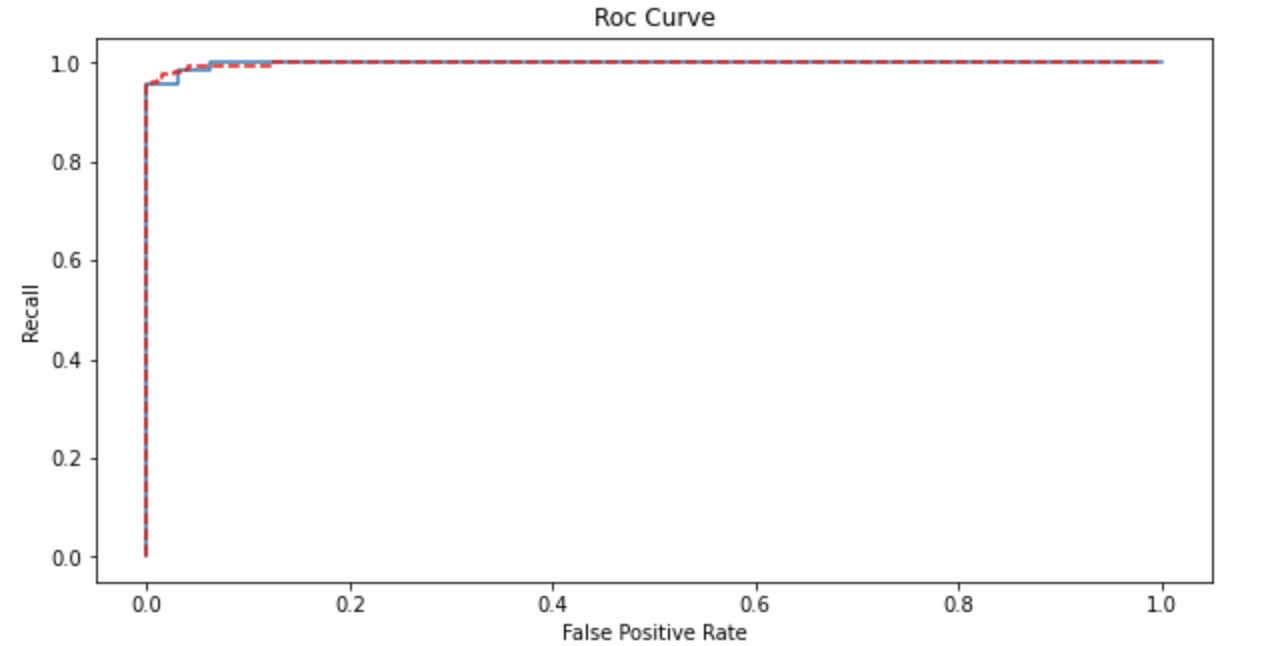
\includegraphics[width=3in]{\FIGDIR/rocsvm.jpg}
\caption{The Roc Curve of ROC}
\label{rocs}
\end{figure}